\chapter{Introduction}
Flow and transport processes between free-flows and porous-media 
flows are common in a wide range of environmental, industrial, civil and medical 
applications.
For example a turbulent air flow has a significant effect on the 
drying rate of an adjacent wet porous-medium like a soil, as studied by  
\textcite{tesi:mosthaf}, \textcite{intro:davarzani} and \textcite  
{tesi:fetzer}.
Although systems like this are very common,	they involve
%This kind of system, in spite of its simplicity, involves
many different physical phenomena that act at 
different scales and
due to concerns of scales and the complexity of the phenomena,
%Thus
a reliable prediction of the evaporation rates is still a challenge. In Figure~\ref{fig:intro} we can 
see a schematic representation of the mechanisms that play a role in such a 
situation, where both transport and thermal effects can be relevant. 
Moreover, considering natural phenomena, an additional difficulty is given by 
the intrinsic uncertainty and heterogeneity of material properties, such as the 
soil porosity, and atmospheric conditions, e.g. the air humidity or the 
solar radiation.
\begin{figure}[ht]
	\centering
	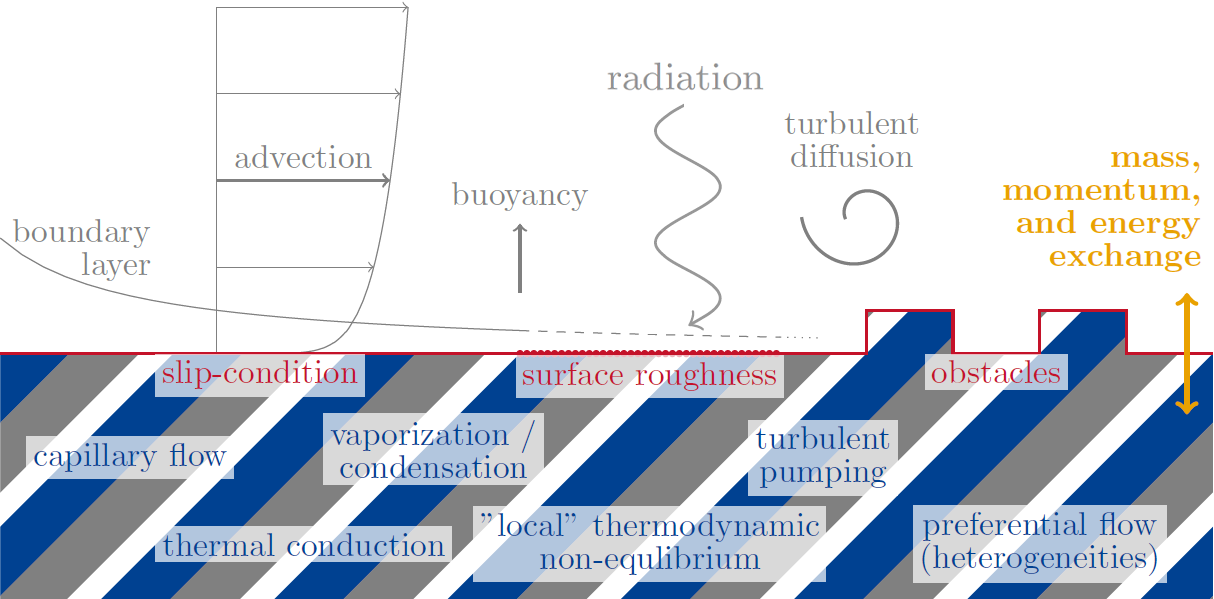
\includegraphics[width=\textwidth]{intropicture2.png}
	\caption[Exchange processes between free and porous-medium 
	flows]{Example of physical phenomena affecting the exchange processes 
		between a free-flow and a porous-medium flow. Figure source: 
		\cite{tesi:fetzer}.}
	\label{fig:intro}
\end{figure}

These studies can be exploited, for example, to better understand the process 
of soil salinization, one of the most serious agricultural problems in 
many arid and coastal areas in the world. It consists in the excessive 
accumulation of salt in the soil pores, with the consequence of a partial or 
complete loss of fertility. A limited amount of salt precipitation in the soil, 
due to evaporation of irrigation water, is inevitable, but a mismanaged irrigation plan could lead to salinity problems in the long term, especially in arid 
areas where irrigation is necessary to increase the production for food supply 
(see \cite{web:fao}). According to \cite{soil:munns}, more than 6\% of world's 
total land area is affected by salinization.
%The part of the soil which is most involved in this problem is the one near the 
%surface, hence it is important to study the interactions between the free-flow 
%and the porous-medium flow that occur there.
The section of a soil profile which is most affected by salinization is the one near the surface, hence the importance of studying the interactions between the free-flow and the porous-medium flow that occur there.
For example, \textcite{intro:salinization} have investigated the application of kinetic 
approaches to describe the salt precipitation in a coupled system.
\begin{figure}
	\centering
	\subfloat[]{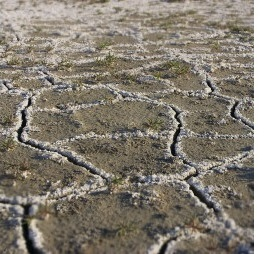
\includegraphics[height=0.22\textheight]{salinity.jpg} 
	\label{fig:soil}}
	\subfloat[]{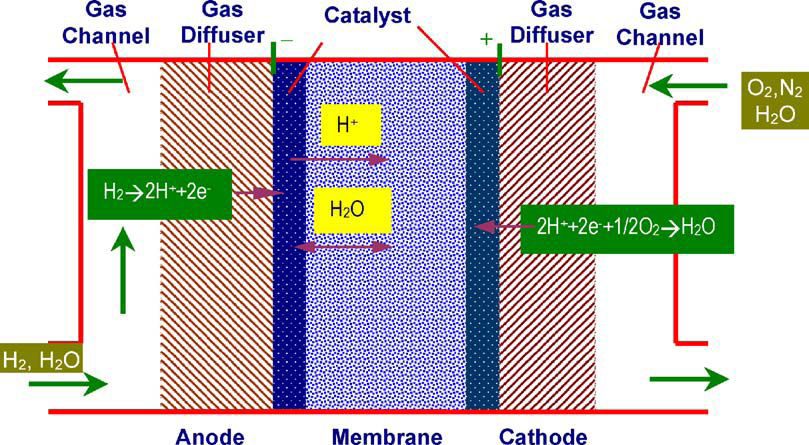
\includegraphics[height=0.22\textheight]{pem.png}\label{fig:pem}}
	\caption[Salt-affected soil and operation principle of PEM fuel 
	cells]{\protect\subref{fig:soil}: Salt-affected soil. Figure source: 
	\cite{web:fao}. \protect\subref{fig:pem}: Operation principle of PEM fuel 
	cells. Figure source: \cite{intro:pemfig}.}
	\label{fig:intro2}
\end{figure}

Switching to a technical framework, Proton Exchange Membrane (PEM) fuel cells 
represent a possible alternative power source that, in particular, could be 
used for transportation. In their design, transport and diffusion phenomena 
through gas channels and gas diffusers play an important role in the 
electrochemical reactions that determine the cell performances and efficiency. 
As we can see in Figure~\ref{fig:intro2}, reactant gases are transported 
through gas channels and supplied at the anode and cathode, then they diffuse 
into porous layers called gas diffusers, that should deliver them uniformly and 
efficiently to the catalyst layers, where reactions take place (see 
\cite{wu:fuelcell}, \cite{tesi:baber} and \cite{tesi:pem}). Protons are 
produced at the anode and transported through the membrane to react with oxygen 
at the cathode and produce water. The water management within the cells is of 
great importance, because it is essential to have a certain level of humidity in 
the membrane in order to facilitate the transport of protons, but an excess of 
water could flood the catalyst layers, with the result of an inhibition of the 
reactions.
Because of the complex and compact geometry of PEM fuel cells, it is generally 
difficult and expensive to take measurements, thus mathematical and numerical 
models are helpful in order to better understand the mechanical, thermal and 
chemical phenomena that take place and this way improve the cell performances 
and lifetime.

Other examples of applications can be found in the fields of refrigeration of 
stored food \cite{intro:food}, cooling systems for aerospace engineering 
\cite{intro:aero}, ventilation of motorcycle helmets \cite{intro:discacim}, 
wind flow around buildings in urban environments \cite{intro:buildings} and 
hemodynamics \cite{intro:med}.

\section{State of the art}
In order to study these processes we focus on
the case of the evaporation from a porous material and we consider
a system that 
involves two subdomains: the upper one with a free-flow and the lower one 
occupied by a porous-medium, as it is represented in Figure~\ref{fig:intro}.
At the interface between the two subdomains there is exchange of mass, momentum 
and energy.

Numerical studies of this coupled system can be performed with a 
\emph{single-domain} approach or with a \emph{two-domain} approach 
\cite{tesi:fetzer}.
Within the single-domain approach, the same equations are solved in the whole 
computational domain, including both the free-flow region and the 
porous-medium. A first possibility is to use the Navier-Stokes equations to model the 
fluid motion and thus to perform a direct numerical simulation (DNS) of the 
whole system. The porous-medium has to be resolved at the pore-scale, thus a 
detailed knowledge of the pore structure and geometry, which is not easy to obtain for real 
materials, is necessary. The computational effort is very high because 
of the strict spatial and temporal requirements of a DNS,
%and it increases even more if the fluid
all of which increase further if the system
is non-isothermal, multi-phase and multi-component. \textcite{intro:dns} and \textcite{intro:dns2} have performed DNS in 
porous-media domains using the lattice Boltzmann method, while \textcite{intro:yang} have performed coupled simulations considering idealised coarse porous materials.
A cheaper possibility for the case of laminar single-phase flows is to employ the Brinkman's equation 
\cite{intro:brinkman}, which is a superposition of the Stokes equations and 
Darcy's law, with a modified viscosity. %:
%\begin{equation}
%	-\nabla \cdot (\tilde{\mu} \nabla \mathbf{v}) + \mu 
%	\mathbf{K}^{-1}\mathbf{v} + \nabla p = \mathbf{f}.
%\end{equation}
Then the transition between the two 
regions can be expressed with a spatial variation of the involved physical 
parameters, either considering a transition region or admitting a discontinuous 
variation at the interface. \textcite{intro:shavit} proposed a modification of 
the Brinkman's equation and applied it to the case of shallow water flows over 
porous surfaces.

Within the two-domain approach, adopted also in this thesis, different sets of 
equations are used in the two subdomains and they are coupled imposing suitable 
conditions at the interface. This allows to keep separated models to describe phenomena that act on different temporal and spatial scales. The free-flow can be modelled with the Stokes 
equations, Navier-Stokes equations or Reynolds Averaged Navier-Stokes (RANS) equations, depending on the flow 
regime. The porous-medium flow, instead, is usually described using a Reference Elementary Volume (REV) scale approach, exploiting the 
Darcy's law or the Forchheimer's law when the Reynolds number is higher or the 
Richards' equation. The interface could also be \emph{complex}, i.e. it could be 
%allowed to store mass, for example to take into account drop formation
adapted to store mass, to, for example, take into account information about the formation of droplets
(see \cite{tesi:baber}).

\textcite{intro:discacim} compared the performances of a single-domain approach exploiting a penalization technique and a 
two-domain approach, using the Navier-Stokes equations and the Forchheimer's 
law to model an incompressible, single-phase, single-component flow. They 
concluded that the former is easier to implement, but the latter more accurately describes the physics of the problem. Alternative approaches may exploit 
pore-networks models in the porous-medium subdomain, that allow to focus on the 
pore scale effects, avoiding the complexity of a DNS (see \cite{paper:kilian}).

\textcite{paper:mosthaf} proposed a Stokes/Darcy coupling concept for multi-phase, 
multi-component, non-isothermal flows. It is based on phenomenological arguments and it tries to be as close as possible to the 
imposition of thermodynamic equilibrium. \textcite{intro:davarzani}, instead, focused on the coupling in case of non-equilibrium conditions among phases.
\textcite{paper:fetzer} generalized the equilibrium concept to the case of 
turbulent flows, in \cite{tesi:fetzer} several turbulence models are tested and 
possible simplifications in the implementation of interface conditions are 
considered. The effects of turbulence, as well as the non-linear inertial 
effects of the Navier-Stokes equations, are sometimes neglected, for 
simplicity, 
but to model natural systems they must be included as they
%play an important role in most of the situations.
affect the physical factors important in most applications.
Another aspect investigated in 
\cite{tesi:fetzer} is the influence of a rough interface between the two 
subdomains. In particular, both the effects of a sand-grain roughness and of 
periodical porous obstacles are studied.
Rough interfaces have been taken into account also in \cite{intro:kuzbek} and \cite{intro:kuz} to analyse heat transfer within a duct, while rough boundaries for free-flows are considered in \cite{lien:obstacles} to study flow paths around buildings, in \cite{intro:limnology}, in a limnological framework, and in \cite{intro:targui} to study heat exchangers.

Theoretical results about the well-posedness can be found in \cite{intro:disca}, for the Stokes/Darcy problem, and in \cite{intro:disca2009}, for the Navier-Stokes/Darcy problem. They are based on classical results for saddle-point problems. Regarding the numerical aspects, many different methods have been employed in literature. In \cite{intro:disca2009} several finite elements choices are considered, in \cite{tesi:mosthaf} the box method is used, while in \cite{tesi:fetzer} the same box method is compared to a combined staggered and collocated finite volumes method. In \cite{intro:disca} an iterative algorithm is proposed in order to decouple the two subdomains, while in \cite{intro:rybak} a temporal decoupling strategy is used.

\section{Content of the thesis}
In this thesis the focus is on the improvement, from the numerical point of view, of the free-flow model with respect to \cite{tesi:fetzer} and on the further investigation of the effects given by a rough interface between the two subdomains.

When the flow is in a turbulent regime, turbulent eddies develop near the interface and 
they cascade through consecutively smaller scales until the kinetic energy 
dissipates into internal thermal energy. Because of their location, they have 
a strong influence on the exchange processes between the two subdomains, so an 
accurate evaluation of their behaviour is of crucial importance. Improvements 
can be obtained with a refinement of the grid, but also by employing 
high order methods. In 
particular, in the discretization of the Navier-Stokes equations using finite 
volumes, the approximation used for the non-linear term 
$\nabla \cdot (\mathbf{v} \mathbf{v}^\mathrm{T})$ plays a key role. A common and easy 
choice is to employ a first order upwind approximation for the 
\emph{transported} velocity, but this option can produce solutions with 
excessive numerical diffusion. Other possibilities are given by high order 
methods 
like the Linear Upwind Differencing (LUD) scheme, the Central Differencing (CD) 
scheme or the Quadratic Upstream Interpolation for Convective Kinetics (QUICK) 
scheme. Under specific conditions, they can produce 
accurate solutions but they have also been shown to be unstable in certain 
situations and to produce overshoots or undershoots that 
may lead to unphysical values of quantities which, for example, have to be 
non-negative (see \cite{main:vermal}). With this in mind, our interest is in 
the Total Variation Diminishing (TVD) methods, a family of methods that has 
been derived with the purpose of providing a solution with a second order 
accuracy, but without any risk of numerical oscillations. They are called also 
high resolution methods \cite{tvd:monotonicity}.

Using this tool, we study a coupled system involving a turbulent free-flow and a porous-medium flow, considering an isothermal, single-phase, single-component fluid. It is a simplified model with respect to the one employed in \cite{tesi:fetzer} to study evaporation processes, but it allows to focus on the fluid mechanical phenomena that occur at the interface. In particular, being in nature the soil surface intrinsically rough, it is important to investigate the effects given by a rough interface, to obtain a deeper understanding of the flow behaviour in this situation. 

The thesis is organized as follows. In Chapter~\ref{chap:equations}, the equations employed in the models will be 
presented, with particular attention to the free-flow equations. In 
Chapter~\ref{chap:discretization}, the finite volume method will be described 
and, in Subsection~\ref{subsec:tvd}, the TVD methods will be introduced. At last, 
in Chapter~\ref{chap:results}, the numerical results will be shown. In 
particular, we will
%see the application of the TVD methods to the Navier-Stokes 
%equations in comparison to 
compare the results obtained with the TVD methods with those obtained
the first order upwind scheme. Then, two tests 
involving turbulent flows are presented and, finally, more complex scenarios involving 
a rough interface, consisting of cavities or porous obstacles, between a free-flow region and a porous-medium is investigated.

The high order methods mentioned above have been implemented in the framework 
of the open-source simulator \DUMUX: DUNE for multi-$\{$phase, component, 
scale, physics, \dots$\}$ flow in porous-media, see \cite{dumux:tutti} and 
\cite{dumux:flemisch}. \DUMUX is an 
additional module of DUNE (Distributed and Unified Numerics Environment, 
\cite{web:dune}) and, through the use of an object-oriented design in 
conjunction with template programming, it provides a C++ environment that 
allows an efficient implementation of numerical models related to porous-media 
flows.

All the source code used for the simulations performed can be 
found at \url{https://git.iws.uni-stuttgart.de/dumux-pub/vescovini2019a}, 
together with the instructions to install the required software.